\chapter{Fundamentação Teórica}

A crescente demanda por sistemas de monitoramento e controle em tempo real tem impulsionado o desenvolvimento de soluções baseadas em sistemas embarcados, especialmente em aplicações voltadas à medição de grandezas elétricas. Esses sistemas permitem a aquisição, processamento e análise de sinais provenientes de sensores, possibilitando maior eficiência, segurança e confiabilidade em instalações elétricas.

Nesse contexto, a correta compreensão dos princípios envolvidos na aquisição de dados, no funcionamento dos sensores elétricos e no processamento de sinais torna-se fundamental para o desenvolvimento de sistemas de monitoramento eficientes. Assim, esta seção apresenta os principais conceitos teóricos relacionados aos sistemas embarcados, à conversão analógico-digital, aos sensores de corrente e tensão, bem como às técnicas de condicionamento e análise de sinais elétricos.

\section{Sistemas Embarcados}
Um sistema embarcado é definido como um sistema computacional inserido e oculto dentro de um equipamento maior, projetado meticulosamente para realizar tarefas específicas, repetitivas e predefinidas. Esta característica contrasta frontalmente com a arquitetura dos computadores de uso geral (como \textit{desktops} e servidores), que são desenhados com alta flexibilidade para suportar uma vasta e imprevisível gama de aplicações orientadas por usuários finais. Os sistemas embarcados operam frequentemente sob restrições severas que desafiam o \textit{design} tradicional, pois possuem recursos limitados de memória e processamento, operam sob orçamentos de energia restritos (frequentemente alimentados por baterias), devem possuir custo de manufatura competitivo e exigem uma confiabilidade operacional quase infalível, visto que muitas vezes não possuem interfaces de usuário complexas para reporte de erros \cite{KLS2018, Immes2024}.

A Figura \ref{fig:arq_embarcado} apresenta a arquitetura típica de um sistema embarcado, composto por três camadas principais: a primeira camada trata-se da unidade de processamento, que é o núcleo do sistema, responsável por executar as tarefas de controle e processamento de dados. A segunda camada é a memória, que armazena o código de programação e os dados necessários para a operação do sistema. A terceira camada é composta pelos periféricos, que incluem os sensores, atuadores e interfaces de comunicação, permitindo a interação do sistema com o ambiente externo. A integração eficiente dessas camadas é crucial para garantir o desempenho e a confiabilidade do sistema embarcado \cite{KLS2018}.

\begin{figure}[!h]
    \centering
    \caption{Arquitetura de um sistema embarcado típico.}
    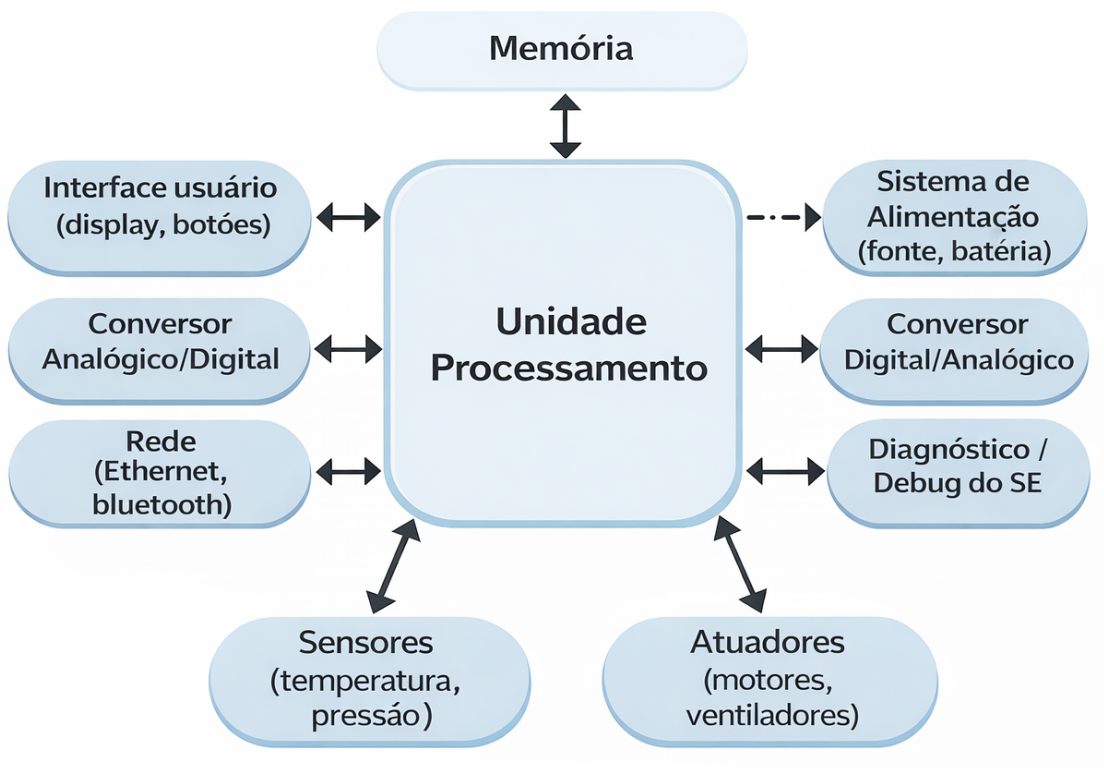
\includegraphics[width=14cm]{figuras/arq_embarcado.png} % Ajuste o nome do arquivo da imagem
    \\ \autoria{Adaptado de \citeonline{KLS2018}.}
    \label{fig:arq_embarcado}
\end{figure}

Uma classificação importante no contexto dos sistemas embarcados está relacionada à criticidade temporal, dando origem aos chamados sistemas de tempo real (\textit{RTOS}). Nesse tipo de sistema, não é suficiente apenas que a tarefa seja executada corretamente do ponto de vista lógico. Além disso, é fundamental que sua execução ocorra dentro de um intervalo de tempo previamente estabelecido, garantindo assim a confiabilidade do sistema \cite{KLS2018}.

Nesse sentido, os sistemas de tempo real podem ser divididos em duas categorias principais. Em primeiro lugar, destacam-se os sistemas de tempo real rígido (\textit{Hard Real-Time}), que apresentam comportamento altamente determinístico. Nesses sistemas, o não cumprimento de um prazo de execução (\textit{deadline}) é inaceitável, podendo resultar em falhas graves, danos ao equipamento ou até mesmo colocar vidas em risco. Por essa razão, são amplamente utilizados em aplicações críticas, como sistemas aeroespaciais, freios ABS e monitores cardíacos \cite{KLS2018}.

Por outro lado, existem os sistemas de tempo real flexível (\textit{Soft Real-Time}), nos quais há uma maior tolerância a atrasos ocasionais na execução das tarefas. Nesses casos, eventuais falhas temporais não comprometem totalmente o funcionamento do sistema, mas podem ocasionar uma degradação na qualidade do serviço. Como exemplo, podem ser citados sistemas multimídia e aplicações de automação não crítica, em que pequenas perdas de desempenho são aceitáveis \cite{KLS2018}.

\section{Microcontroladores}
O núcleo de processamento lógico de um sistema embarcado moderno é, quase na sua totalidade, materializado por um microcontrolador. Este dispositivo é um circuito integrado denso que encapsula, em uma única pastilha de silício, uma Unidade Central de Processamento (CPU), memória de programa (geralmente \textit{Flash} ou ROM), memória de dados (RAM), portas de entrada e saída (E/S), \textit{timers}, e múltiplos periféricos de comunicação. O mercado de semicondutores oferece uma vasta gama de opções de fabricantes, diferenciando-se fundamentalmente pela capacidade de processamento, consumo energético e, de forma primária, por sua arquitetura interna de barramentos e execução de instruções. Apesar da enorme diversidade evolutiva na computação desde meados do século XX, duas arquiteturas seminais ditaram os rumos do \textit{design} de processadores e microcontroladores: a arquitetura de Von Neumann e a arquitetura de Harvard \cite{Oliveira2006}.

Conforme ilustrado na Figura \ref{fig:von_neumann}, a arquitetura de Von Neumann, cujos fundamentos teóricos foram delineados pelo eminente físico e matemático húngaro-americano John von Neumann em seu histórico documento \textit{First Draft of a Report on the EDVAC}, publicado em 30 de junho de 1945, é caracterizada por um paradigma unificado de memória. A estrutura geral proposta possui uma memória principal única que armazena, indistintamente, dados operacionais e instruções de programa. Esta arquitetura utiliza o mesmo barramento físico para o transporte de ambos. Embora esta convergência simplifique o \textit{design} da matriz do circuito e da placa de circuito impresso, ela introduz um gargalo estrutural severo conhecido academicamente como o "Gargalo de Von Neumann". Como a Unidade Lógica e Aritmética (ULA) e a Unidade de Controle não podem realizar a busca (\textit{fetch}) de uma instrução e a leitura ou escrita de um dado operacional de forma estritamente simultânea, o processamento ocorre obrigatoriamente de forma sequencial. Os ciclos do processador são desperdiçados em estados de espera (\textit{wait states}). Microprocessadores baseados nesta arquitetura são tradicionalmente associados ao modelo \textit{CISC} (\textit{Complex Instruction Set Computer}), visando maximizar o trabalho por instrução devido à lentidão do acesso à memória \cite{Neumann1945, Patterson2014}.

\begin{figure}[!h]
    \centering
    \caption{Arquitetura de Von Neumann.}
    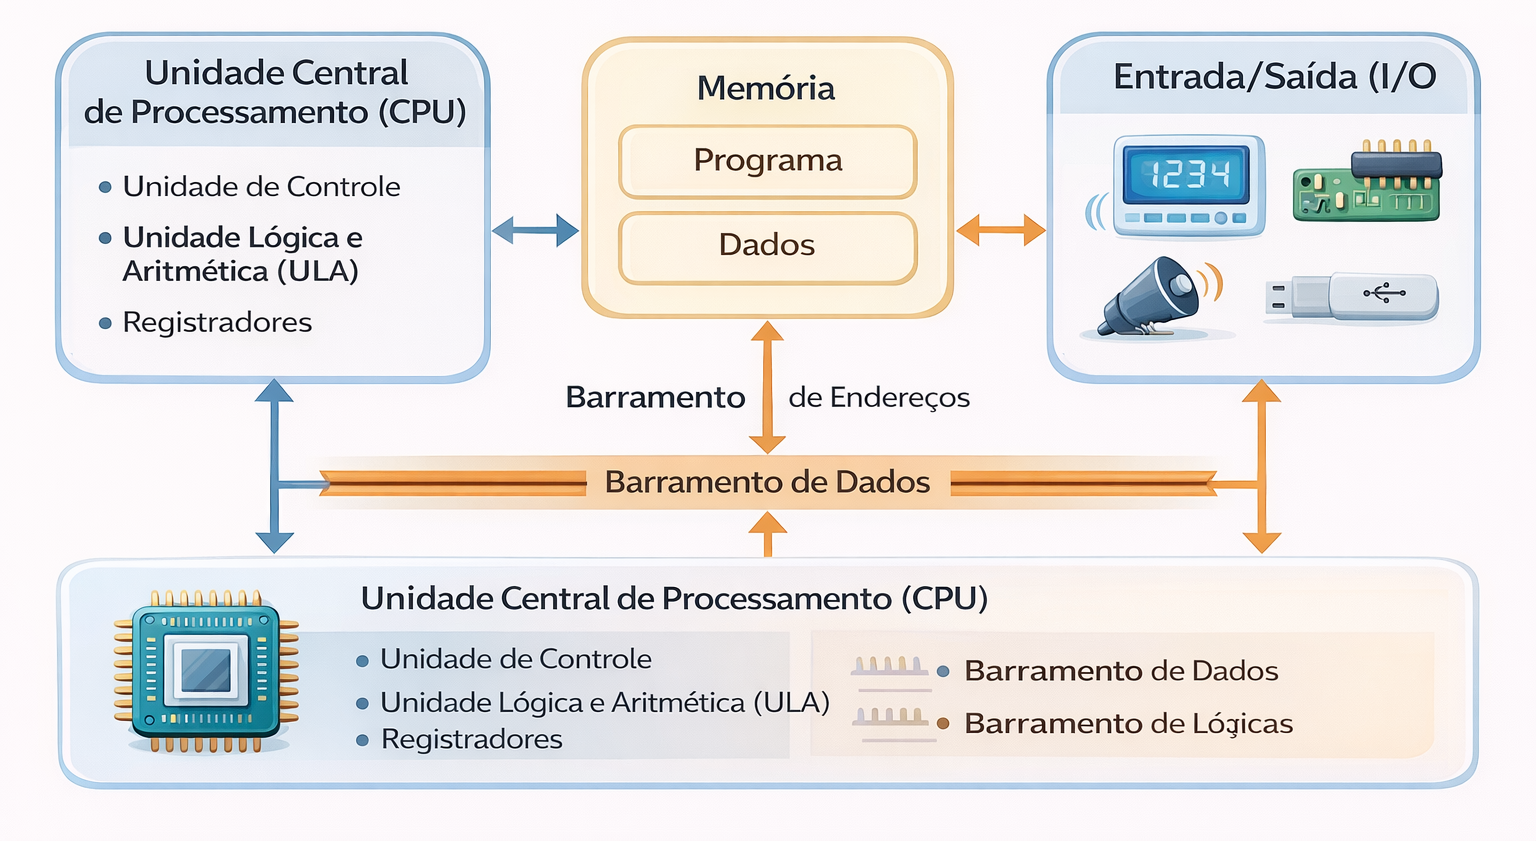
\includegraphics[width=12cm]{figuras/von_neumann.png}
    \\ \autoria{Autoria Própria.}
    \label{fig:von_neumann}
\end{figure}

Em contraste direto, a arquitetura de Harvard, apresentada na Figura \ref{fig:harvard}, resolve o impasse de concorrência ao isolar fisicamente e logicamente os domínios de informação. Ela possui duas memórias distintas e independentes: uma dedicada exclusivamente à retenção do programa (instruções) e outra dedicada aos dados temporários da aplicação. A principal característica que define a arquitetura Harvard é a provisão de conjuntos de fios independentes (dois barramentos separados) interligando a CPU a cada tipo de memória. Com base nessa separação, o processador conquista a liberdade de acessar ambas as memórias de maneira simultânea. Isso viabiliza técnicas avançadas como o \textit{pipelining} (linha de montagem de instruções), em que, durante o exato ciclo de máquina em que o processador executa uma instrução matemática complexa, o barramento de programa já está buscando a instrução subsequente na memória \textit{Flash}, operando de forma exponencialmente mais eficiente e rápida que sua contraparte de Von Neumann. Grande parte dos microcontroladores de alto desempenho empregados na moderna aquisição de sinais — como as famílias ARM Cortex e microcontroladores baseados em núcleos \textit{RISC} (\textit{Reduced Instruction Set Computer}) — operam sob princípios de Harvard ou variações híbridas (Harvard modificada) \cite{Oliveira2006, Yiu2013, Patterson2014}.

\begin{figure}[!h]
    \centering
    \caption{Arquitetura Harvard.}
    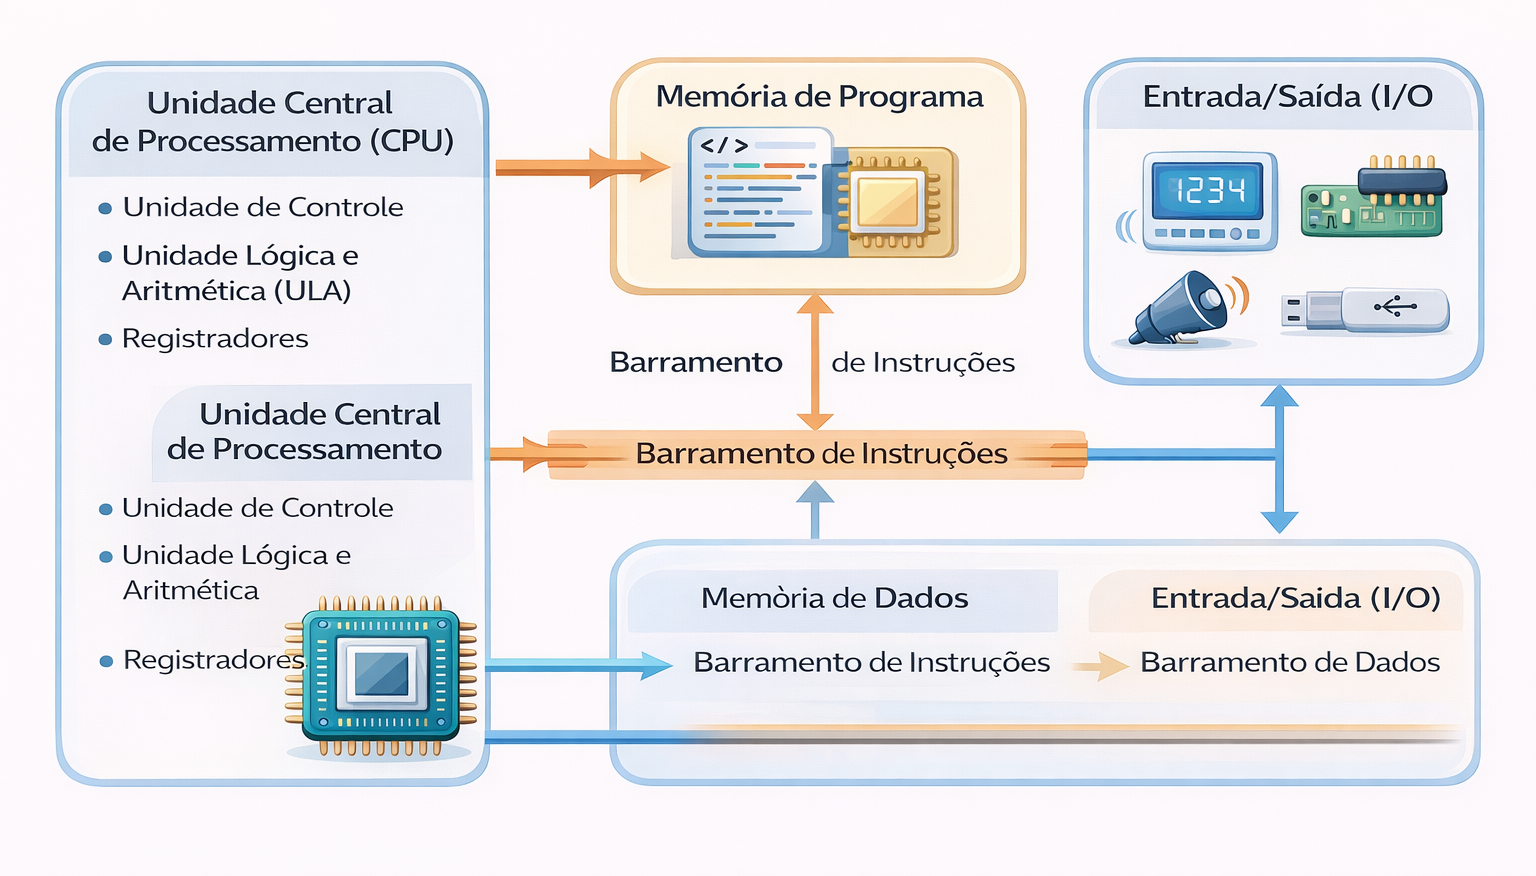
\includegraphics[width=12cm]{figuras/harvard.png}
    \\ \autoria{Autoria Própria.}
    \label{fig:harvard}
\end{figure}

Para uma compreensão estruturada, a Tabela \ref{quad:arquiteturas} ilustra as diferenças que definem a adequação destas arquiteturas aos projetos de eletrônica embarcada.

\begin{quadro}[htb]
    \centering
    \caption{Arquiteturas de Von Neumann x Harvard}
    \label{quad:arquiteturas}
    \begin{tabular}{|l|p{5cm}|p{5cm}|}
        \hline
        \textbf{Característica Estrutural} & \textbf{Arquitetura de Von Neumann} & \textbf{Arquitetura de Harvard} \\
        \hline
        \textbf{Organização de Memória} & Espaço unificado para código e dados. & Espaços de memória fisicamente separados. \\
        \hline
        \textbf{Barramentos} & Um único barramento compartilhado. & Barramentos independentes para instruções e dados. \\
        \hline
        \textbf{Acesso Simultâneo} & Impossível (Gargalo de Von Neumann). & Possível, permitindo alta concorrência (\textit{pipelining}). \\
        \hline
        \textbf{Complexidade de Hardware} & Menor, resultando em chips de silício menores. & Maior, devido à duplicação da malha de roteamento. \\
        \hline
        \textbf{Paradigma de Instruções} & Frequentemente associado a arquiteturas CISC. & Tipicamente associado a arquiteturas RISC. \\
        \hline
        \textbf{Desempenho Geral} & Menor \textit{throughput} por ciclo de \textit{clock}. & Alto \textit{throughput}, execução próxima a 1 instrução/ciclo. \\
        \hline
    \end{tabular}
    \autoria{Elaborado pelo autor.}
\end{quadro}
\subsection{Conversor Analógico-Digital (ADC)}
O ADC cumpre a função de receber níveis variáveis de tensão gerados por transdutores ambientais e transformá-los em palavras digitais inteligíveis para a Unidade Lógica e Aritmética. No âmbito dos microcontroladores comerciais aplicados em métricas de energia e automação, a topologia de conversão predominante pelo equilíbrio entre velocidade, custo e resolução é o ADC de Aproximações Sucessivas (\textit{SAR - Successive Approximation Register}). 

A estrutura de \textit{hardware} subjacente, ilustrada na Figura \ref{fig:adc_sar}, envolve tipicamente quatro blocos funcionais: um circuito de amostragem e retenção (\textit{Sample-and-Hold}), um comparador de tensão analógico, um Conversor Digital-Analógico (DAC) interno de alta velocidade, e o próprio registrador de aproximação sucessiva acoplado à lógica de controle \cite{Kester2005, AnalogDevices2025}.

\begin{figure}[!h]
    \centering
    \caption{Diagrama de blocos do ADC de Aproximações Sucessivas (SAR).}
    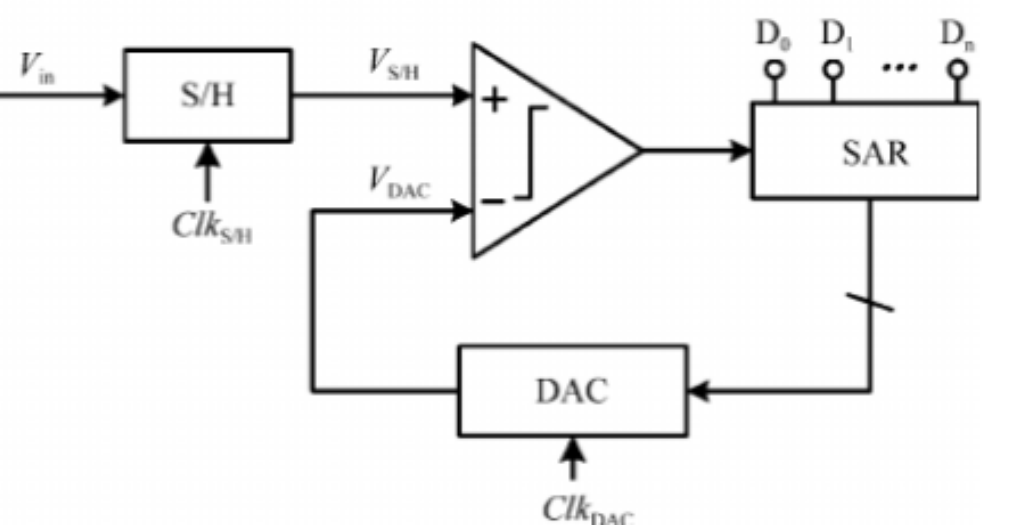
\includegraphics[width=12cm]{figuras/adc_sar.png}
    \\ \autoria{\citeonline{AnalogDevices2025}.}
    \label{fig:adc_sar}
\end{figure}

A dinâmica de conversão procede da seguinte maneira: primeiro, evitar que flutuações bruscas no sinal de entrada causem erros imprevisíveis durante o processo. O circuito \textit{Sample-and-Hold} carrega um capacitor interno que retém momentaneamente a tensão de entrada estática na porta do comparador. Simultaneamente, o algoritmo SAR força o \textit{bit} mais significativo (\textit{MSB - Most Significant Bit}) do registrador interno para o nível lógico alto ('1'), definindo o valor binário inicial exatamente na metade do fundo de escala (por exemplo, 10000000 em um sistema de 8 \textit{bits}). O DAC interno converte essa palavra digital em uma tensão analógica física, igual à metade da tensão de referência ($V_{ref}/2$). O comparador então confronta essa tensão gerada pelo DAC com a tensão analógica real amostrada.

Se a tensão retida de entrada for maior que a tensão do DAC, a tentativa foi um sucesso parcial, e o \textit{MSB} permanece em '1'. Se for menor, a estimativa do DAC foi muito alta, e o \textit{MSB} é revertido para '0'. Este processo de "testar, comparar e manter ou descartar" repete-se sucessivamente, \textit{bit} a \textit{bit}, movendo-se para os \textit{bits} menos significativos (\textit{LSB}) até que a combinação binária resulte em uma tensão de saída do DAC que se alinhe com a máxima proximidade possível à tensão original de entrada. O número de ciclos de \textit{clock} necessários para finalizar a conversão é rigidamente atrelado ao número de \textit{bits} do conversor, tornando o tempo de conversão constante, um atributo altamente desejável para processamento em tempo real \cite{Kester2005, ScienceDirect2025}.

A qualidade e a utilidade prática do processo de quantização são ditadas por um parâmetro primordial: a resolução do conversor analógico-digital. A resolução é invariavelmente estabelecida pelo número finito de \textit{bits} de saída ($n$), que determina a quantidade de degraus de quantização discretos nos quais a faixa de tensão analógica contínua será subdividida. A menor variação de tensão possível que o microcontrolador é teoricamente capaz de distinguir é referida como passo de quantização, \textit{quantum} ou \textit{LSB}, expresso algebricamente como:

\begin{equation}
    Quantum = \frac{V_{ref}}{2^n}
\end{equation}

em que $V_{ref}$ é a tensão analógica máxima permitida pelo limite superior do conversor. A literatura exemplifica que, ao mensurar grandezas fisiológicas ou elétricas que sofrem condicionamento prévio, a correta escolha desta resolução é mandatória \cite{Patterson2014, Kester2005}.

A precisão sistêmica, entretanto, transcende o número de \textit{bits}. A conversão de tensão do mundo real depende profundamente da estabilidade absoluta do barramento de referência analógica (AREF) e do \textit{offset} introduzido pelos circuitos passivos. Ruídos acoplados à linha $V_{ref}$ propagam-se instantaneamente, distorcendo os múltiplos de contagem. Na engenharia de \textit{software}, a tradução da contagem numérica devolvida ao formato de ponto flutuante utilitário processa-se pela equação inversa \cite{Kester2005, ScienceDirect2025}:

\begin{equation}
    V_{entrada} = \frac{Contagem \times V_{ref}}{2^{n}-1}
\end{equation}

\section{Aquisição de Dados}
A aquisição de dados em sistemas de instrumentação corresponde, do ponto de vista da teoria de sinais, à operação de amostragem: a conversão de um sinal de tempo contínuo $x(t)$ em uma sequência de tempo discreto $x[n]$, obtida pela coleta de valores de $x(t)$ em múltiplos inteiros de um intervalo de amostragem $T$, de modo que:

\begin{equation}
    x[n] = x(nT)
\end{equation}

sendo $T$ o período de amostragem determinado pelo \textit{timer} de \textit{hardware} do microcontrolador \cite{Haykin2001}.

A operação de amostragem gera, portanto, um sinal de tempo discreto a partir de um sinal de tempo contínuo, sendo amplamente empregada para permitir a manipulação do sinal por computadores e microprocessadores em sistemas de comunicação, controle e processamento de sinais. O efeito da amostragem pode ser avaliado formalmente pela relação entre a Transformada de Fourier de Tempo Discreto (DTFT) do sinal amostrado $x[n]$ e a Transformada de Fourier contínua (FT) do sinal original $x(t)$ \cite{Haykin2001}.

\section{Teorema de Nyquist-Shannon e o Fenômeno de Aliasing}
Segundo \citeonline{Haykin2001}, a representação por FT do sinal amostrado no domínio da frequência consiste em uma versão periodicamente replicada do espectro do sinal original, com réplicas espaçadas de $\omega_{s}=2\pi/T$ radianos por segundo ao longo do eixo de frequências. Essa replicação espectral é consequência direta da multiplicação do sinal contínuo por um trem de impulsos, matematicamente denominado de pente de Dirac no domínio do tempo.

Para que o sinal de tempo contínuo original possa ser reconstruído de maneira exata a partir de suas amostras, é necessário que as réplicas espectrais não se sobreponham. Essa condição é satisfeita quando a frequência de amostragem $f_{s}=1/T$ é maior ou igual ao dobro da componente de maior frequência $f_{max}$ presente no espectro do sinal:

\begin{equation}
    f_{s} \ge 2f_{max}
\end{equation}

A frequência limiar $f_{s}/2$ é denominada frequência de Nyquist. Quando essa condição é violada, isto é, quando o sinal contém componentes espectrais acima da frequência de Nyquist, as réplicas se sobrepõem à faixa de frequência principal em um fenômeno denominado \textit{aliasing} (subamostragem). 

A Figura \ref{fig:nyquist_aliasing} ilustra o efeito da amostragem no domínio da frequência. Em (d), observa-se que quando $\omega_{s}<2W$, as réplicas do espectro se sobrepõem, resultando no fenômeno de \textit{aliasing}. Nessa situação, componentes de alta frequência se disfarçam como componentes falsas de baixa frequência no sinal digital resultante, tornando impossível, por processamento subsequente, separar a perturbação do sinal original. Uma vez instalado o \textit{aliasing}, a contaminação espectral é irreversível no domínio digital \cite{Haykin2001}.

\begin{figure}[!h]
    \centering
    \caption{Efeito da amostragem no espectro: (a) sinal original; (b) amostragem adequada; (c) limite de Nyquist; (d) \textit{aliasing} por subamostragem.}
    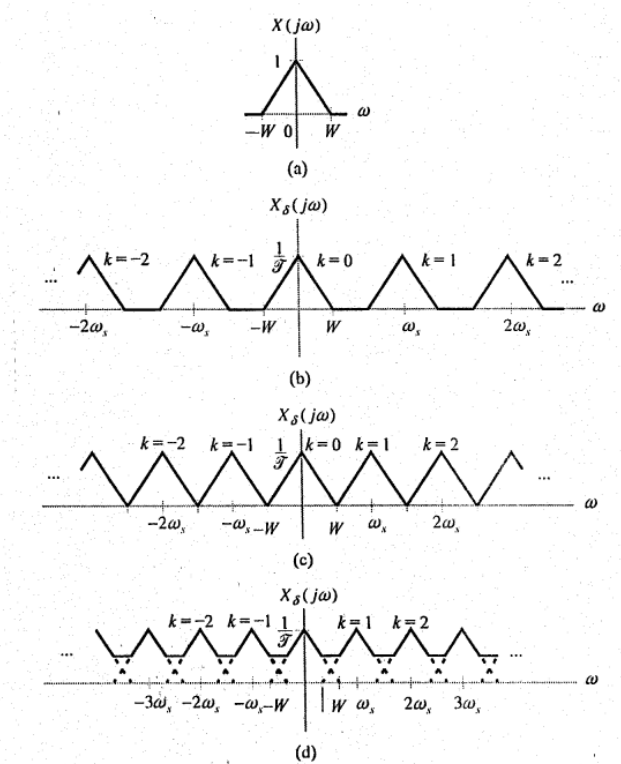
\includegraphics[width=12cm]{figuras/aliasing.png}
    \\ \autoria{\citeonline{Haykin2001}.}
    \label{fig:nyquist_aliasing}
\end{figure}

No contexto prático da medição de grandezas elétricas em redes de distribuição operando à frequência fundamental de 50 Hz ou 60 Hz, a presença de dispositivos de eletrônica de potência impõe harmônicos de ordem superior ($3^a, 5^a, 7^a$) ao sinal. Para garantir a fidelidade da aquisição, faz-se necessário o emprego de filtros analógicos passa-baixa (filtros \textit{anti-aliasing}) na entrada do conversor A/D, os quais limitam a banda do sinal antes da amostragem, além da adoção de taxas de amostragem suficientemente elevadas — tipicamente entre 1000 Hz e 3000 Hz em aplicações embarcadas de medição de energia \cite{Haykin2001}.

\section{Condicionamento de Sinais}
Os sinais provenientes diretamente dos sensores analógicos não são adequados para leitura por microcontroladores, principalmente devido às limitações de nível de tensão e à presença de componentes alternados. Enquanto a rede elétrica opera com sinais senoidais que assumem valores positivos e negativos, os sistemas embarcados trabalham, em geral, com níveis de tensão positivos e limitados (como 3,3 V ou 5 V) \cite{Alexander2013}. Dessa forma, torna-se necessário um estágio de condicionamento de sinais para adequar essas grandezas ao intervalo de operação do conversor analógico-digital (ADC) \cite{OpenEnergy2019}.

\subsection{Resistor de Carga}
No caso de sensores de corrente com saída em corrente, como o SCT-013-000, o primeiro estágio de condicionamento consiste na utilização de um resistor de carga (\textit{burden resistor}), responsável por converter a corrente do secundário em uma tensão proporcional, conforme a Lei de Ohm \cite{Alexander2013, OpenEnergy2019}:

\begin{equation}
    V = R_{burden} \cdot I_{s}
\end{equation}

O dimensionamento desse resistor deve ser feito de forma que o sinal de saída utilize ao máximo a faixa do ADC, sem ultrapassar seus limites \cite{OpenEnergy2019, OpenEnergy2015}. Para isso, considera-se a corrente máxima no primário e a relação de transformação do sensor.

A corrente de pico no primário pode ser obtida a partir do valor RMS \cite{Alexander2013}:

\begin{equation}
    I_{pico} = I_{RMS} \cdot \sqrt{2}
\end{equation}

Já a corrente no secundário é dada por \cite{OpenEnergy2019}:

\begin{equation}
    I_{s} = \frac{I_{pico}}{N}
\end{equation}

Assim, o valor do resistor de carga pode ser estimado por \cite{OpenEnergy2019, OpenEnergy2015}:

\begin{equation}
    R_{burden} = \frac{V_{ref}}{2 \cdot I_{s}}
\end{equation}

Em que $V_{ref}$ representa a tensão de referência do ADC. Na prática, escolhe-se um valor comercial ligeiramente inferior ao calculado, evitando saturação do sinal \cite{OpenEnergy2015}.

\subsection{Offset DC e Polarização}
Como o sinal proveniente dos sensores é alternado e centrado em zero, ele não pode ser aplicado diretamente ao ADC \cite{OpenEnergy2019}. Para resolver esse problema, adiciona-se um nível DC ao sinal, deslocando-o para a faixa positiva. Esse processo é realizado por meio de um divisor resistivo, que cria uma tensão de referência igual à metade da tensão de alimentação \cite{Alexander2013, OpenEnergy2019}:

\begin{equation}
    V_{offset} = \frac{V_{cc}}{2}
\end{equation}

Esse ponto funciona como novo referencial para o sinal alternado, permitindo que ele oscile dentro da faixa do ADC \cite{OpenEnergy2019}. Além disso, utiliza-se um capacitor em série ou em paralelo, dependendo da topologia, para bloquear a componente DC indesejada e permitir apenas a passagem da componente alternada, formando um circuito do tipo RC \cite{Alexander2013}.

\subsection{Amplificação de Sinais}
Em alguns casos, o sinal obtido apresenta baixa amplitude, o que compromete a resolução do ADC. Nesses casos, utiliza-se um amplificador operacional para aumentar a amplitude do sinal \cite{Sedra2017}.

Para uma configuração não inversora, o ganho do amplificador é dado por \cite{Sedra2017}:

\begin{equation}
    A_{v} = 1 + \frac{R_{2}}{R_{1}}
\end{equation}

Na prática, entretanto, amplificadores operacionais não são ideais. Fatores como tensão de \textit{offset}, ruído e limitações de ganho podem introduzir erros na medição \cite{Sedra2017}. Por esse motivo, módulos comerciais como o ZMPT101B já incluem circuitos de ajuste, como \textit{trimpots}, que permitem calibrar o ganho e minimizar esses efeitos \cite{DataCapture2023}. Dessa forma, o condicionamento de sinais garante que os sinais provenientes dos sensores sejam adequadamente ajustados em amplitude e nível de tensão, permitindo sua correta leitura pelo sistema embarcado.

\section{Grandezas Elétricas em Sistemas Digitais}
Em sistemas modernos de medição elétrica baseados em processamento digital, diferentemente dos métodos analógicos tradicionais, as grandezas são obtidas a partir de algoritmos numéricos aplicados a sinais discretizados. Nesse contexto, normas como a IEEE 1459-2010 estabelecem diretrizes para o cálculo das potências elétricas em ambientes não senoidais \cite{IEEE2010}, utilizando amostras digitais de tensão $v[k]$ e corrente $i[k]$, adquiridas por conversores analógico-digitais (ADC).

\subsection{Medidores Convencionais}
Instrumentos convencionais que não utilizam cálculo RMS verdadeiro (\textit{True RMS}) operam com base na média retificada do sinal, aplicando um fator de correção fixo, válido apenas para ondas senoidais puras \cite{Alexander2013, Dugan2012}. Em sistemas reais, em que há presença de harmônicas, ruídos e cargas não lineares (como inversores e retificadores), essa aproximação gera erros significativos \cite{Dugan2012, Akagi2007}. Por isso, o uso de algoritmos \textit{True RMS} torna-se essencial para medições confiáveis.

\subsection{Sistemas Não Senoidais e Abordagens Avançadas}
O modelo clássico de potência elétrica, baseado nas grandezas potência ativa (P), reativa (Q) e aparente (S), é amplamente utilizado em sistemas de medição devido à sua simplicidade e aplicabilidade em condições senoidais ideais \cite{Alexander2013}. Nessas condições, as relações matemáticas tradicionais, como:

\begin{equation}
    S = V_{RMS} \cdot I_{RMS} \quad \text{e} \quad Q = \sqrt{S^{2} - P^{2}}
\end{equation}

são válidas e representam adequadamente o comportamento físico do sistema \cite{IEEE2010, Alexander2013}. 

Entretanto, em redes elétricas modernas, é comum a presença de cargas não lineares, como inversores, retificadores e fontes chaveadas, que introduzem distorções harmônicas nas formas de onda de tensão e corrente \cite{Dugan2012}. Nesses casos, as relações clássicas deixam de representar completamente os fenômenos envolvidos, especialmente no que se refere à potência reativa e ao fator de potência \cite{IEEE2010, Akagi2007}.

Com o objetivo de superar essas limitações, surgiram abordagens mais avançadas, como a Teoria da Potência Conservativa (TPC), que propõe uma decomposição mais rigorosa das componentes de corrente e potência, permitindo a separação entre parcelas associadas à energia útil, armazenamento e distorção harmônica \cite{Tenti2011, Paredes2012}. No entanto, a implementação completa dessas metodologias exige maior complexidade computacional e processamento adicional, sendo mais comum em analisadores de qualidade de energia de alto desempenho \cite{Tenti2011}.

\section{Qualidade de Energia Elétrica}
A qualidade de energia elétrica (QEE) está relacionada à capacidade do sistema elétrico fornecer tensão, corrente e frequência dentro de condições adequadas, garantindo o funcionamento correto dos equipamentos conectados. Quando esses parâmetros apresentam desvios em relação aos valores nominais, podem ocorrer falhas, redução de desempenho ou até danos às cargas \cite{Filho2010}.

No Brasil, a regulamentação da qualidade de energia é definida pela ANEEL por meio do PRODIST, que estabelece critérios, limites e classificações para os principais fenômenos que afetam o fornecimento \cite{ANEEL2021}.

\subsection{Classificação dos Fenômenos}
De acordo com o PRODIST, os fenômenos de qualidade de energia podem ser classificados principalmente em variações de tensão de curta duração e de longa duração. As variações de curta duração incluem eventos como interrupções, afundamentos e elevações de tensão, enquanto as de longa duração estão associadas a condições de subtensão e sobretensão. Esses distúrbios podem ter origem tanto no sistema elétrico quanto nas próprias instalações dos consumidores, dependendo do tipo de carga e das condições de operação \cite{Jr2012}.

\subsection{Afundamento de Tensão}
Entre os fenômenos de QEE, o afundamento de tensão é um dos mais frequentes e relevantes. Ele é caracterizado por uma redução temporária da tensão eficaz, normalmente associada a faltas no sistema elétrico ou à partida de cargas de grande porte. Esse fenômeno ocorre devido à circulação de correntes elevadas na rede, que provocam quedas de tensão nas impedâncias do sistema. Dessa forma, quanto maior a corrente de falta, mais acentuado será o afundamento observado \cite{Jr1986}.

A severidade do afundamento depende de fatores como:
\begin{itemize}
    \item distância do ponto de falta;
    \item impedância do sistema;
    \item tipo de perturbação.
\end{itemize}

Além disso, o afundamento pode ser caracterizado por três parâmetros principais: magnitude (tensão residual), duração e, em alguns casos, o desequilíbrio entre fases. A Figura \ref{fig:afundamento} ilustra um exemplo de afundamento de tensão, evidenciando a redução temporária da tensão eficaz e a subsequente recuperação ao valor nominal.

\begin{figure}[!h]
    \centering
    \caption{Exemplo de afundamento de tensão em sistema trifásico.}
    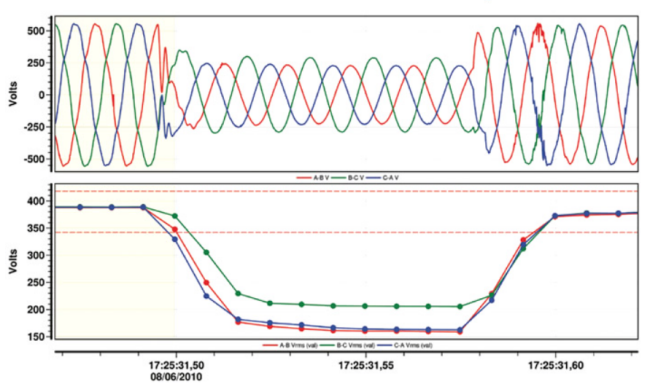
\includegraphics[width=14cm]{figuras/afundamento.png}
    \\ \autoria{\citeonline{ElectricService2026}.}
    \label{fig:afundamento}
\end{figure}


\subsection{Impactos nas Instalações}
Os afundamentos de tensão podem causar diversos impactos, principalmente em equipamentos sensíveis, como inversores de frequência, sistemas de automação e computadores. Entre os principais efeitos, destacam-se:
\begin{itemize}
    \item desligamentos inesperados;
    \item falhas em processos automatizados;
    \item perdas de produção.
\end{itemize}

\section{Aprendizado de Máquina}
O Aprendizado de Máquina (\textit{Machine Learning} - ML) é um subcampo da Inteligência Artificial voltado ao desenvolvimento de algoritmos que aprendem padrões a partir de dados, sem que as regras de decisão sejam explicitamente programadas \cite{Bishop2006}. Os algoritmos são geralmente classificados em três paradigmas: aprendizado supervisionado, não supervisionado e por reforço \cite{Hastie2009}.

No aprendizado supervisionado, o modelo é treinado a partir de pares entrada-saída $(x_{i},y_{i})$, buscando estimar uma função $f:x\mapsto y$ que minimize o erro entre a resposta predita e a real — paradigma mais adequado ao contexto deste trabalho \cite{Bishop2006}.

\subsection{Redes Neurais Artificiais e a Célula GRU}
As Redes Neurais Artificiais (RNAs) são modelos computacionais inspirados no sistema nervoso biológico, estruturados como composições de transformações parametrizadas cujos pesos são ajustados durante o treinamento \cite{Bishop2006}. A unidade fundamental é o neurônio artificial, que computa um potencial de ativação $v_{k}$ a partir de suas entradas e aplica uma função não linear $\varphi(\cdot)$ para produzir sua saída \cite{Bishop2006}:

\begin{equation}
    v_{k} = \sum_{j=1}^{N}w_{kj}x_{j}+b_{k}, \quad y_{k} = \varphi(v_{k})
\end{equation}

As Redes Neurais Recorrentes (RNRs) estendem esse modelo para o processamento de sequências temporais, mantendo um estado interno de memória atualizado a cada passo de tempo \cite{Haykin2001}. Contudo, sofrem do problema do desvanecimento do gradiente em sequências longas \cite{Goodfellow2016}. A \textit{Gated Recurrent Unit} (GRU), proposta por \citeonline{Cho2014}, mitiga essa limitação por meio de dois mecanismos de porta: a porta de atualização $z_{t}$ e a porta de redefinição $r_{t}$ — que controlam seletivamente quais informações passadas devem ser retidas ou descartadas. O estado oculto é atualizado como \cite{Cho2014}:

\begin{equation}
    h_{t} = (1-z_{t}) \odot h_{t-1} + z_{t} \odot \tilde{h}_{t}
\end{equation}

em que $\tilde{h}_{t}$ é o estado candidato, calculado a partir da entrada atual e do estado anterior filtrado por $r_{t}$. Em comparação com a arquitetura \textit{LSTM}, a GRU possui menor número de parâmetros, resultando em menor custo computacional \cite{Goodfellow2016}.

\subsection{Máquina de Vetores de Suporte}
A Máquina de Vetores de Suporte (\textit{Support Vector Machine} - SVM) é um algoritmo supervisionado que determina um hiperplano de decisão ótimo, maximizando a margem de separação entre as classes \cite{Bishop2006}. Para dados não linearmente separáveis, emprega o \textit{kernel trick}, que mapeia as amostras para um espaço de dimensão superior no qual a separação linear torna-se possível \cite{Hastie2009}.

\subsection{K-Nearest Neighbors}
O \textit{K-Nearest Neighbors} (KNN) é um classificador não-paramétrico que armazena as amostras de treinamento e prediz a classe de uma nova amostra por votação majoritária entre os K vizinhos mais próximos, segundo uma métrica de distância \cite{Bishop2006, Hastie2009}. Seu desempenho depende da escolha adequada de K e da métrica utilizada.

\subsection{Árvores de Decisão e Métodos de Ensemble}
As Árvores de Decisão particionam recursivamente o espaço de características, mas tendem a apresentar alta variância \cite{Hastie2009}. Os métodos de \textit{Ensemble Learning} combinam múltiplos modelos para produzir estimadores mais robustos \cite{Goodfellow2016}. O \textit{Random Forest} constrói um conjunto de árvores descorrelacionadas via \textit{Bagging}, selecionando aleatoriamente subconjuntos de características em cada divisão de nó \cite{Hastie2009}. 

Já o \textit{CatBoost} é fundamentado em \textit{Gradient Boosting}, construindo o modelo sequencialmente, onde cada nova árvore corrige os erros residuais da anterior \cite{Hastie2009}. O \textit{CatBoost} introduz o modo \textit{Ordered Boosting}, que evita o vazamento de dados durante o cálculo dos gradientes, mitigando o \textit{overfitting} \cite{Goodfellow2016}.

\subsection{Otimização e Validação}
A seleção dos hiperparâmetros é etapa determinante para a qualidade do modelo \cite{Goodfellow2016}. A Otimização Bayesiana constrói um modelo probabilístico da função objetivo para guiar a busca nas regiões mais promissoras do espaço de hiperparâmetros, sendo mais eficiente que métodos exaustivos como o \textit{Grid Search} \cite{Hastie2009}. A robustez dos modelos é avaliada por meio da Validação Cruzada Aninhada (\textit{Nested Cross-Validation}), que emprega um laço interno para otimização dos hiperparâmetros e um laço externo para avaliação imparcial do desempenho, prevenindo o vazamento de dados \cite{Goodfellow2016}.

\subsection{Métricas de Avaliação}
O desempenho dos classificadores é quantificado por métricas derivadas da Matriz de Confusão \cite{Hastie2009}. As principais são: Acurácia, razão entre predições corretas e total de amostras; Precisão, qualidade das predições positivas; \textit{Recall}, capacidade de detectar amostras positivas; e \textit{F1-Score}, média harmônica entre Precisão e \textit{Recall} \cite{Bishop2006}. Complementarmente, a Curva ROC e sua área (\textit{Area Under the Curve} - AUC) fornecem uma avaliação independente do limiar de decisão, variando de 0,5 (aleatório) a 1,0 (perfeito) \cite{Hastie2009}.